\documentclass[../../main/main.tex]{subfiles}
\graphicspath{{./figures/}}

\dominitoc
\faketableofcontents

% \renewcommand{\mtcSfont}{\small\bfseries}
% \renewcommand{\mtcSSfont}{\footnotesize}
\mtcsettitle{minitoc}{}
\mtcsetrules{*}{off}

\makeatletter
\renewcommand{\@chapapp}{Mécanique -- chapitre}
\renewcommand{\chaplett}{M}
\makeatother

% \toggletrue{student}
\toggletrue{corrige}
% \renewcommand{\mycol}{black}
% \renewcommand{\mycol}{gray}

\hfuzz=5.002pt

\begin{document}
\setcounter{chapter}{2}

% \settype{book}
% \settype{prof}
% \settype{stud}

\chapter{Mouvements courbes}

\vspace*{\fill}

\begin{tcn}(appl)<ctc>"somm"'t'{Sommaire}
	\let\item\olditem
	\vspace{-15pt}
	\minitoc
	\vspace{-25pt}
\end{tcn}

\begin{tcn}[sidebyside]
	(appl)<ctb>"how"'t'{Capacités exigibles}
	\begin{itemize}[label=\rcheck]
		\item Identifier les degrés de liberté d'un mouvement. Choisir un système
		      de coordonnées adapté au problème.

		      % \item Systèmes de coordonnées cartésiennes, cylindriques et sphériques.
		      %
		\item Vitesse et accélération dans le repère de Frenet pour une
		      trajectoire plane.

		\item Coordonnées cylindriques~: exprimer à partir d'un schéma le
		      déplacement élémentaire, construire le trièdre local associé et en
		      déduire géométriquement les composantes du vecteur vitesse.

		\item Établir les expressions des composantes des vecteurs position,
		      déplacement élémentaire, vitesse et accélération en coordonnées
		      cylindriques.
	\end{itemize}
	\tcblower
	\begin{itemize}[label=\rcheck]
		\item Mouvement circulaire uniforme et non uniforme~: exprimer les
		      composantes du vecteur position, du vecteur vitesse et du vecteur
		      accélération en coordonnées polaires planes.

		\item Exploiter les liens entre les composantes du vecteur accélération,
		      la courbure de la trajectoire, la norme du vecteur vitesse et sa
		      variation temporelle.

		\item Établir l’équation du mouvement du pendule simple. Justifier
		      l’analogie avec l'oscillateur harmonique dans le cadre de
		      l'approximation linéaire.
	\end{itemize}
\end{tcn}

\vspace*{\fill}
\newpage
\vspace*{\fill}

%\vspace{-15pt}
\begin{tcn}[%
		sidebyside, fontupper=\small, fontlower=\small
	](appl)<ctb>"chek"'t'{L'essentiel}
	\tce{defi}
	% \tce{rapp}
	% \tce{loi}
	\tce{prop}
	\tce{demo}
	\tce{theo}
	\tce{prev}
	% \tce{coro}
	% \tce{inte}
	% \tce{impl}
	% \tce{tool}
	% \tce{nota}
	% \tce{appl}
	% \tce{rema}
	% \tce{exem}
	% \tce{ror}
	% \tce{impo}
	\tcblower
	% \tce{defi}
	\tce{rapp}
	% \tce{prop}
	% \tce{theo}
	% \tce{loi}
	% \tce{coro}
	% \tce{demo}
	% \tce{inte}
	% \tce{impl}
	% \tce{nota}
	\tce{appl}
	\tce{rema}
	\tce{exem}
	\tce{tool}
	\tce{ror}
	\tce{impo}
\end{tcn}

\vspace*{\fill}

\newpage

\section{Mouvement courbe dans un plan}
\subsection{Position en coordonnées polaires}

\begin{tcb*}[sidebyside, righthand ratio=.35](defi)
	{Repère polaire et vecteur position}
	Le repère polaire est constitué d'une origine O autour de laquelle sont
	définis deux vecteurs $\ur$ et $\ut$ tels que~:
	\begin{itemize}
		\item \psw{$\ur$ dans la direction $\OM$}
		\item \psw{$\ut \perp \ur$ dans le sens direct}
		\item[m][15] \psw{%
			      \[
				      \boxed{\OM(t) = r(t)\ur}
				      \qet
				      \boxed{\norm{\OM}(t) = r(t)}
			      \]
		      }%
		      \vspace{-15pt}
	\end{itemize}
	\begin{center}
		\fatbox{\textbf{$\ur$ et $\ut$ dépendent de $\th(t)$ donc du temps}}
	\end{center}
	\tcblower
	\begin{center}
		\sswitch{%
			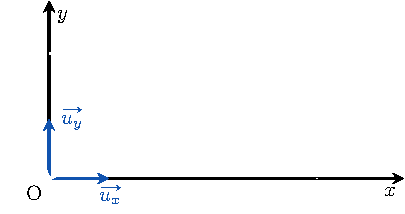
\includegraphics[width=\linewidth]{pos_pol_stud}
		}{%
			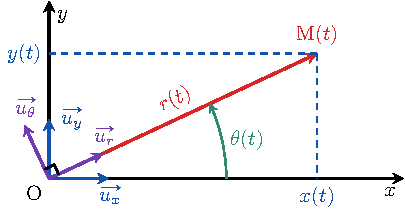
\includegraphics[width=\linewidth]{pos_pol_prof}
		}%
		\vspace{-15pt}
		\captionof{figure}{Polaires}
	\end{center}
\end{tcb*}

\begin{tcb*}(impo)<lftt>{Variables vs.\ coordonnées}
	Il faut opérer la distinction entre les \textbf{variables} servant à repérer
	le point et les \textbf{coordonnées} dans la base de projection. Ici, les
	variables sont $r(t)$ et $\th(t)$, mais dans la base $(\ur,\ut)$, on a
	\[
		\OM(t) = \mqty(r(t)\\0) = r(t)\ur
		\qMath{\textbf{ET PAS}}
		\dcancel{%
		\OM(t) = \mqty(r(t)\\\th(t)) = r(t)\ur +
		\underbracket[1pt]{\th(t)\ut}_{\mathclap{\text{pas homogène~!}}}
		}
	\]
	\vspace{-15pt}
\end{tcb*}

\begin{tcb*}(prop){Lien polaires/cartésiennes}
	Les vecteurs $\ur$ et $\ut$ variables se décomposent sur $\ux$ et $\uy$
	fixes tels que
	\[
		\psw{\boxed{\ur = \cos(\th(t))\ux + \sin(\th(t))\uy}}
		\qet
		\psw{\boxed{\ur = -\sin(\th(t))\ux + \cos(\th(t))\uy}}
	\]
	d'où en cartésiennes pour un point M~:
	\[
		\psw{%
			x(t) = r(t)\cos(\th(t))
		}%
		\qet
		\psw{%
			y(t) = r(t)\sin(\th(t))
		}%
		\qso
		\psw{%
			\norm{\OM}(t) = r(t) = \sqrt{x(t)^2 + y(t)^2}
		}%
	\]
\end{tcb*}

\begin{tcb*}(demo){Lien polaires/cartésiennes}
  On projette les vecteurs de la base polaire sur la base cartésienne en
  appliquer la méthode de vraisemblance ou par définition du produit
  scalaire, d'où la propriété. On a alors~:
  \psw{%
    \begin{gather*}
      \OM(t) = r(t)\ur
      \Lra
      \OM(t) =
      \underbracket[1pt]{r(t)\cos(\th(t))}_{=x(t)}\ux +
      \underbracket[1pt]{r(t)\sin(\th(t))}_{=y(t)}\uy
      \\\Ra
      \norm{\OM}(t) =
      \sqrt{x(t)^2 + y(t)^2} =
      \sqrt{r(t)^2\underbracket[1pt]{\pa{\cos^2(\th(t)) + \sin^2(\th(t))}}_{=1}}
      = r(t) \qed
    \end{gather*}
  }%
  \vspace{-15pt}
\end{tcb*}

\vspace{-15pt}
\subsection{Variation temporelle des vecteurs de base}
\begin{tcb*}[breakable](tool){Dérivée composée en physique}
	En physique, on a l'habitude (mathématiquement valable) de penser les dérivées
	comme des fractions. Ainsi, on peut traiter la dérivée d'une composition en
	faisant intervenir d'autres dérivée par une écriture fractionnaire. Par
	exemple~:
	\psw{%
		\begin{gather*}
			\dv{t}\/(\cos(\theta(t))) =
      \dv{\th}{t} \dv{\th} (\cos(\theta(t))) =
      -\tp(t) \sin(\theta(t))
		\end{gather*}
	}%
  \vspace{-15pt}
\end{tcb*}

\begin{tcb*}(prop){Dérivées de $\protect\ur$ et $\protect\ut$}
  La variation temporelle des vecteurs de la base polaire est~:
  \[
    \psw{%
      \boxed{\dv{\ur}{t} = \tp(t)\ut}
    }%
    \qet
    \psw{%
      \boxed{\dv{\ut}{t} = -\tp(t)\ur}
    }%
  \]
  \vspace{-15pt}
\end{tcb*}

\begin{tcb*}[breakable](demo){Dérivées de $\protect\ur$ et $\protect\ut$}
  % On peut travailler géométriquement ou par le calcul, en repassant en
  % coordonnées cartésiennes.
  \tcbsubtitle{\fatbox{\textbf{Géométriquement}}}
  \begin{isd}[interior hidden, righthand ratio=.3](demo)
  On représente les deux vecteurs après un petit temps $\dd{t}$, c'est-à-dire
  augmentés d'un angle $\dd{\th}$~:
      \begin{align*}
        \psw{%
          \dd{\ur} = \underbracket[1pt]{\norm{\ur}}_{=1}\cdot \dd{\th} \ut
        }%
        \qeta
        \psw{%
          \dd{\ut} = \underbracket[1pt]{\norm{\ut}}_{=1}\cdot \dd{\th} (-\ur)
        }%
        \\\beforetext{Soit}
        \psw{%
          \dv{\ur}{t} = \dv{\th}{t}\ut
        }%
        \qeta
        \psw{%
          \dv{\ut}{t} = -\dv{\th}{t}\ur
        }%
        \qed
      \end{align*}
    \tcblower
    \begin{center}
      \sswitch{%
        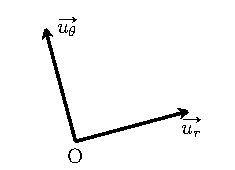
\includegraphics[width=\linewidth]{pol_dur_stud}
      }{%
        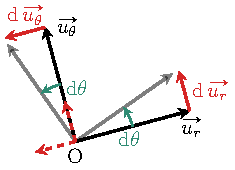
\includegraphics[width=\linewidth]{pol_dur_prof}
      }%
      \vspace{-15pt}
      \captionsetup{justification=centering}
      \captionof{figure}{\\$\dd\protect\ur$ et $\dd\protect\ut$}
    \end{center}
  \end{isd}
  \tcblower
  \tcbsubtitle{\fatbox{\textbf{Mathématiquement}}}
  On part des décompositions dans la base cartésienne et on dérive~:
  \smallbreak
  \begin{isd}[interior hidden](demo)
    \tcbsubtitle{\fatbox{\!$\ur$}}
    \vspace{-15pt}
    \psw{%
      \small
      \begin{DispWithArrows*}[fleqn, mathindent=0pt]
        \ur
        & =
        \cos(\th)\ux + \sin(\th)\uy
        \CArrow{$\dv{t}\/(\cdot)$}
        \\\Lra
        \dv{\ur}{t}
        & =
        \dv{\cos(\th)}{t}\ux + \dv{\sin(\th)}{t}\uy
        \Arrow{Composée}
        \\\Lra
        \dv{\ur}{t}
        & =
        -\tp\sin(\th)\ux + \tp\cos(\th)\uy
        \Arrow{Factorisa$^\circ$}
        \\\Lra
        \dv{\ur}{t}
        & =
          \tp \underbracket[1pt]{\left(-\sin(\th)\ux + \cos(\th)\uy\right)}_{= \ut}
        \Arrow{Identifica$^\circ$}
        \\\Lra
        \dv{\ur}{t}
        & =
        \tp\ut
        \qed
      \end{DispWithArrows*}
    }%
    \vspace{-15pt}
    \tcblower
    \tcbsubtitle{\fatbox{\!$\ut$}}
    \vspace{-15pt}
    \psw{%
      \small
      \begin{DispWithArrows*}[fleqn, mathindent=0pt]
        \ut
        & =
        -\sin(\th)\ux + \cos(\th)\uy
        \CArrow{$\dv{t}\/(\cdot)$}
        \\\Lra
        \dv{\ut}{t}
        & =
        \dv{(-\sin(\th))}{t}\ux + \dv{\cos(\th)}{t}\uy
        \Arrow{Composée}
        \\\Lra
        \dv{\ut}{t}
        & =
        -\tp\cos(\th)\ux - \tp\sin(\th)\uy
        \Arrow{Facto.}
        \\\Lra
        \psw{\dv{\ut}{t}}
        & =
          -\tp \underbracket[1pt]{\left(\cos(\th)\ux + \sin(\th)\uy\right)}_{= \ur}
        \Arrow{Identif.}
        \\\Lra
        \dv{\ut}{t}
        & =
        -\tp\ur
        \qed
      \end{DispWithArrows*}
    }%
    \vspace{-15pt}
  \end{isd}
\end{tcb*}


\subsection{Déplacement élémentaire en polaires}
\begin{tcb*}(prop){Déplacement élémentaire polaire}
	En coordonnées polaires, le déplacement élémentaire s'exprime
	\psw{\[\boxed{\dd\OM = \dd r\ur + r(t)\dd\th\ut}\]}
	\vspace{-15pt}
\end{tcb*}

% On a toujours $\dd\OM = \OM(t+\dt) - \OM(t)$. On trouve son expression
% géométriquement~:

\begin{tcb*}[sidebyside, righthand ratio=.40](demo)
  {Déplacement élémentaire polaire}
  On trouve la composante de $\dd{\OM}$ sur $\ur$ en \xul{fixant $\th$} et on
  \xul{incrémente la variable $r$ de $\dd{r}$}.
  \begin{center}
    La distance ainsi obtenue est \xul{\psw{$\dd{r}$ sur $\ur$.}}
  \end{center}
  \bigbreak
  On trouve la composante de $\dd{\OM}$ sur $\ut$ en \xul{fixant $r$} et on
  \xul{incrémente la variable $\th$ de $\dd{\th}$}.
  \begin{center}
    La distance ainsi obtenue est \xul{\psw{$r(t)\dd{\th}$ sur $\ut$.}}
  \end{center}
  \tcblower
  \begin{center}
    \sswitch{%
      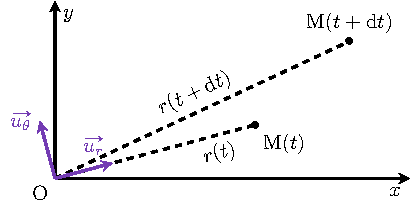
\includegraphics[width=\linewidth]{pol_dom_stud}
    }{%
      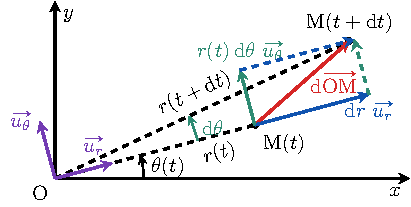
\includegraphics[width=\linewidth]{pol_dom_prof}
    }%
    \vspace{-15pt}
    % \captionsetup{justification=centering}
    \captionof{figure}{$\dd{\protect\OM}$ polaire}
  \end{center}
\end{tcb*}

\subsection{Vitesse en coordonnées polaires}

\begin{tcb*}(prop){Vitesse en coordonnées polaires}
	La vitesse en coordonnées polaires s'écrit
	\psw{\[\boxed{\vf(t) = \rp(t)\ur + r(t)\tp(t)\ut}\]}
	\vspace{-15pt}
\end{tcb*}

\begin{tcb*}(demo)<lftt>{Vitesse en polaires}
Ici aussi, il y a deux manières d'obtenir l'expression de la vitesse.
\tcbsubtitle{\fatbox{\textbf{Dérivée}}}
\vspace{-15pt}
		\psw{%
	\begin{gather*}
			\vf(t) =
      \dv{\OM}{t} =
      \dv{(r(t)\ur)}{t}
			\Lra
			\vf(t) = \rp(t)\ur + r(t)\dv{\ur}{t}
			\Lra
			\vf(t) = \rp(t)\ur + r(t)\tp(t)\ut
      \qed
	\end{gather*}
		}%
  \vspace{-15pt}
  \tcblower
  \tcbsubtitle{\fatbox{\textbf{Rapport}}}
  \psw{%
    \[
      \vf(t) =
      \dv{\OM}{t} =
      \frac{\dd{r}\ur + r(t) \dd{\th}\ut}{\dd{t}} =
      \dv{r}{t} \ur + r(t) \dv{\th}{t}\ut
      \qed
    \]
  }%
  \vspace{-15pt}
\end{tcb*}

\subsection{Accélération}
\begin{tcb*}*(demo)<lftt>"ror"{Accélération en polaires}
Par définition,
\psw{%
      \begin{gather*}
      \af = \dv{\vf}{t} =
      \dv{\tikzmark{DV}}{t}
      \left(
      \rp\tikzmark{RP}(t)\ur\tikzmark{UR} +
      r\tikzmark{R}(t)\tp\tikzmark{TP}(t)\ut\tikzmark{UT}
      \right)
      \\
      \Lra
      \af =
      \psw[orchid]{\rpp(t)}\ur +
      \rp(t) \underbracket[1pt]{\psw[cornflowerblue]{\dv{\ur}{t}}}_{= \tp(t)\ut} +
      \psw[limegreen]{\rp(t)}\tp(t)\ut +
      r(t)\psw[orange]{\tpp(t)}\ut +
      r(t)\tp(t) \underbracket[1pt]{\psw[firebrick]{\dv{\ut}{t}}}_{= -\tp(t)\ur}
  \qed
    \end{gather*}
}%
  \vspace{-35pt}

	\tikz[remember picture, overlay]
	\draw[-stealth, transform canvas={yshift=6pt}, color=\sswitch{white}{orchid}]
	(pic cs:DV) to [out=90, in=90] ([shift={(-3pt,3pt)}]pic cs:RP)
	;
	\tikz[remember picture, overlay]
	\draw[-stealth, transform canvas={yshift=6pt}, color=\sswitch{white}{cornflowerblue}]
	(pic cs:DV) to [out=90, in=90] ([shift={(-6pt,6pt)}]pic cs:UR)
	;
	\tikz[remember picture, overlay]
	\draw[-stealth, transform canvas={yshift=6pt}, color=\sswitch{white}{limegreen}]
	(pic cs:DV) to [out=90, in=90] ([shift={(-3pt,3pt)}]pic cs:R)
	;
	\tikz[remember picture, overlay]
	\draw[-stealth, transform canvas={yshift=6pt}, color=\sswitch{white}{orange}]
	(pic cs:DV) to [out=90, in=90] ([shift={(-3pt,6pt)}]pic cs:TP)
	;
	\tikz[remember picture, overlay]
	\draw[-stealth, transform canvas={yshift=6pt}, color=\sswitch{white}{firebrick}]
	(pic cs:DV) to [out=90, in=90] ([shift={(-6pt,6pt)}]pic cs:UT)
	;

\end{tcb*}

\begin{tcb*}(prop){Accélération en coordonnées polaires}
	Finalement, la vitesse en coordonnées polaires s'écrit
	\psw{
		\[
			\boxed{
				\af = \left( \rpp -r\tp^2 \right)\ur + \left( 2\rp\tp+r\tpp \right)\ut
			}
		\]
	}
	\vspace{-15pt}
\end{tcb*}

\section{Exemples de mouvements plans}
\subsection{Mouvement circulaire}

\begin{tcb*}(defi)<lftt>{Mouvement circulaire}
	Un mouvement est dit \textbf{circulaire} s'il se fait dans un plan, à une
	distance de l'axe de rotation $r$ constante, soit
	\psw{%
		\[
			r(t) = \cte = R
		\]
	}%
	\vspace{-25pt}
\end{tcb*}

\begin{tcb}(impl)<lftt>{Mouvement circulaire}
  Dans ce cas-là, on a
\[
  \psw{\OM(t) = R\ur}
  \qet
  \psw{\rp(t) = 0 = \rpp(t)}
\]
En notant $\w(t) = \tp(t)$ la vitesse angulaire, la vitesse et l'accélération
donnent
\[
  \psw{\boxed{\vf(t) = R\w(t)\ut}}
  \qet
  \psw{\boxed{\af(t) = -R\w^2(t)\ur + R\wp(t)\ut}}
\]
\vspace{-35pt}
\end{tcb}

% \begin{tcb*}(impo){$\w$ en mécanique vs.\ $\w$ en filtrage}
% 	Bien que les symboles des variables soient les mêmes, les deux grandeurs
% 	décrites n'ont \textbf{rien à avoir} entre elles~:
% 	\begin{itemize}
% 		\item $\w$ en filtrage est la \textit{pulsation}~;
% 		\item $\w$ en mécanique est la \textit{vitesse angulaire}.
% 	\end{itemize}
% 	Cependant, les deux ont la \textbf{même unité}, les $\si{rad.s^{-1}}$,
% 	puisqu'elles décrivent bien la variation d'un angle/d'une phase dans le temps.
% \end{tcb*}

\vspace{-15pt}

\subsection{Mouvement circulaire uniforme}
\begin{tcb*}(defi)<lftt>{Mouvement circulaire uniforme}
	Un mouvement est dit \textbf{circulaire \textit{uniforme}} si c'est un
	mouvement circulaire ($r(t) = \cte$) à \textit{vitesse angulaire
		constante}, soit
	\psw{%
		\[
				r(t) = R
        \qet
				\tp(t) = \w_0
		\]
	}%
  \vspace{-25pt}
\end{tcb*}

\begin{tcb}(impl)<lftt>{Mouvement circulaire uniforme}
  Dans ce cas, $\rp = 0 = \rpp$ mais également $\tpp = 0$, donc la vitesse et
  l'accélération donnent
\[
  \psw{\boxed{\vf(t) = R\w_0\ut}}
  \qet
  \psw{\boxed{\af(t) = -R\w_0{}^2\ur}}
\]
\vspace{-25pt}
\end{tcb}

% \begin{tcb*}(ror){Mouvement circulaire uniforme}
% 	Dans le cas du mouvement circulaire uniforme,
% 	\begin{itemize}
% 		\item Le vecteur vitesse est selon $\ut$ et est de norme constante,
% 		      égale à $R\w_0$~;
% 		\item Le vecteur accélération pointe vers le centre et est de norme
%       constance, égale à $\DS R\w_0{}^2 = \frac{v^2}{R}$.
% 	\end{itemize}
% \end{tcb*}

% \begin{tcb}*(expe)<itc>"trans"{Transition}
% 	Si la trajectoire d'un objet change de courbure, il peut être fastidieux de
% 	travailler avec les coordonnées polaires~: on utilisera alors un repère
% 	attaché à l'objet.
% \end{tcb}

\vspace*{-25pt}

\subsection{Repère de \textsc{Frenet}}

\begin{tcb*}[sidebyside, righthand ratio=.4](defi){Repère de \textsc{Frenet}}
  Soit un point M sur une trajectoire courbe d'origine O. On approxime sa
  trajectoire à un instant $t$ par son \textbf{cercle osculateur}, de \textbf{rayon
  de courbure} $R(t)$. D'où le repère de \textsc{Frenet}~:
    \begin{itemize}
      \item \psw{$\vv{u_T}$ tangent à la trajectoire en M~;}
      \item \psw{%
              $\vv{u_N} \perp \vv{u_T}$ dirigé vers le centre.
            }%
    \end{itemize}
    $\gamma(t) = 1/R(t)$ s'appelle la \textbf{courbure} de
  la trajectoire.
    \tcblower
    \begin{center}
      \sswitch{%
        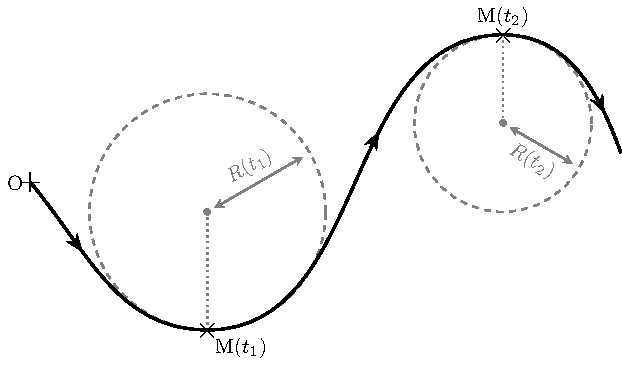
\includegraphics[width=\linewidth]{frenet_stud}
      }{%
        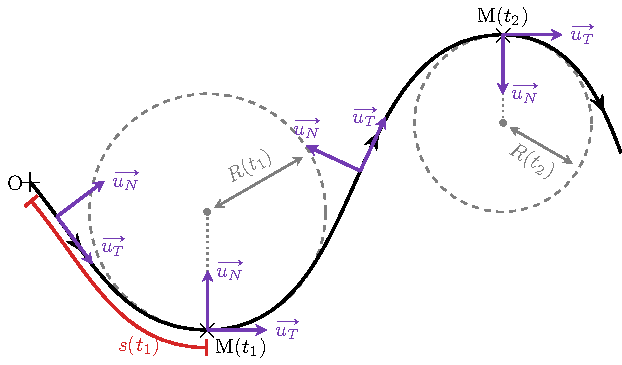
\includegraphics[width=\linewidth]{frenet_prof}
      }%
      \vspace{-15pt}
      \captionof{figure}{\textsc{Frenet}}
    \end{center}
\end{tcb*}

\begin{tcb*}(prop){Vitesse et accélération \textsc{Frenet}}
  La vitesse et l'accélération dans le repère mobile de \textsc{Frenet}
  s'expriment~:
  \[
    \psw{\boxed{\vf(t) = v(t) \vv{u_T}}}
    \qet
    \psw{\boxed{\af(t) = \vp(t) \vv{u_T} + \frac{v(t)^2}{R(t)}\vv{u_N}}}
  \]
\end{tcb*}

\begin{tcb*}(demo)<lftt>{Vitesse et accélération \textsc{Frenet}}
    Soit $s(t)$ la distance parcourue sur la courbe de la trajectoire $\Cc$
    depuis l'origine O. On l'appelle \textbf{abscisse curviligne}, telle que
    \[
      s(t) = \int_{\Cc} \dd{s}
    \]
    \tcbsubtitle{\fatbox{\textbf{Vitesse}}}
    \vspace{-15pt}
    \psw{%
          \begin{gather*}
          \dd{\OM} =
          \OM (t + \dd{t}) - \OM(t) =
          \OM(t+\dd{t}) + \vv{\Mr(t)\Or} =
          \vv{\Mr(t)\Mr(t+\dd{t})} = \dd{s} \vv{u_T}
          \\\Lra
          \vv{u_T} = \dv{\OM}{s}
          \Ra 
          \vf(t) =
          \dv{\OM}{t} =
          \underbracket[1pt]{\dv{s}{t}}_{= v(t)}
          \underbracket[1pt]{\dv{\OM}{s}}_{= \vv{u_T}}
          \qed
        \end{gather*}
    }%
    \vspace{-15pt}
    \tcbsubtitle{\fatbox{\textbf{Accélération}}}
    \vspace{-15pt}
    \begin{isd}[interior hidden, righthand ratio=.3](demo)
      \begin{gather*}
            \beforetext{De plus,}
    \psw{%
            \af(t) = \dv{\vf}{t} = \vp(t)\vv{u_T} + v(t) \dv{\vv{u_T}}{t}
    }%
    \\
        \beforetext{Or,}
        \psw{%
                  \dd{\vv{u_T}} =
                \dd{\th} \vv{u_N}
                \qet
                \dd{s} = R(t) \dd{\th}
                \qso
                \frac{\dd{s}}{R(t)}\vv{u_N}
        }%
        \\
        \psw{%
          \Lra
          \dv{\vv{u_T}}{t} = \frac{1}{R(t)} \dv{s}{t} \vv{u_N}
          \Lra
          \boxed{\dv{\vv{u_T}}{t} = \frac{v(t)}{R(t)}\vv{u_N}} 
        }%
        \\
        \beforetext{D'où}
        \psw{%
                        \boxed{\af(t) = \vp(t)\vv{u_T} + \frac{v(t)^2}{R(t)}\vv{u_N}}
                      \qed
        }%
      \end{gather*}
      \tcblower
      \begin{center}
        \sswitch{%
                  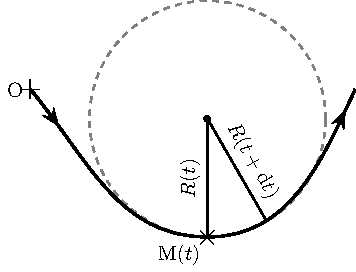
\includegraphics[width=\linewidth]{frenet_demo_stud}
        }{%
        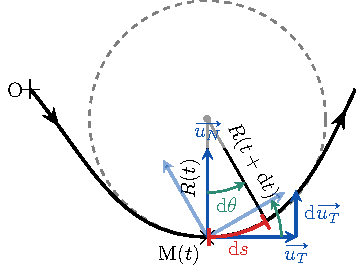
\includegraphics[width=\linewidth]{frenet_demo_prof}
        }%
        \vspace{-15pt}
        \captionof{figure}{$\dd{\protect\vv{u_T}}$}
      \end{center}
    \end{isd}
\end{tcb*}

\begin{tcb*}(rema)<lftt>{Cas limites repère de \textsc{Frenet}}
	\begin{itemize}
		\item On retrouve le mouvement rectiligne uniforme avec $R = +\infty \Lra
			      \gamma = 0$, puisqu'on a alors
		      \[\af = \dv{v}{t}\vv{u_T}\]
		      avec $\vv{u_T}$ dans le sens de la trajectoire.

		\item On retrouve également le mouvement circulaire puisque dans ce cas la
		      trajectoire \textbf{est} le cercle osculateur, donc $\vv{u_T} = \ut$ et
		      $\vv{u_N} = -\ur$.
	\end{itemize}
\end{tcb*}

\section{Application~: pendule simple}

\subsection{Tension d'un fil}
\begin{tcb*}(defi){Tension d'un fil}
	Un point matériel M accroché à un fil tendu subit de la part de ce fil une
	force appelée \textbf{tension du fil} et notée $\Tf$ telle que
	\psw{
		\[\boxed{\Tf = \norm{\Tf}\ur}\]
	}
	avec $\ur$ un vecteur unitaire dirigé \textbf{du point M vers le fil} et
	$\norm{\Tf}$ la norme de la tension du fil.
\end{tcb*}

\begin{tcb*}[bld](ror){Condition de support}
	\begin{center}
		La \textbf{condition de tension} est \psw{$\norm{\Tf} > 0$.}
	\end{center}
	\smallbreak
	\noindent
	\begin{minipage}{0.45\linewidth}
		\begin{center}
			\sswitch{
				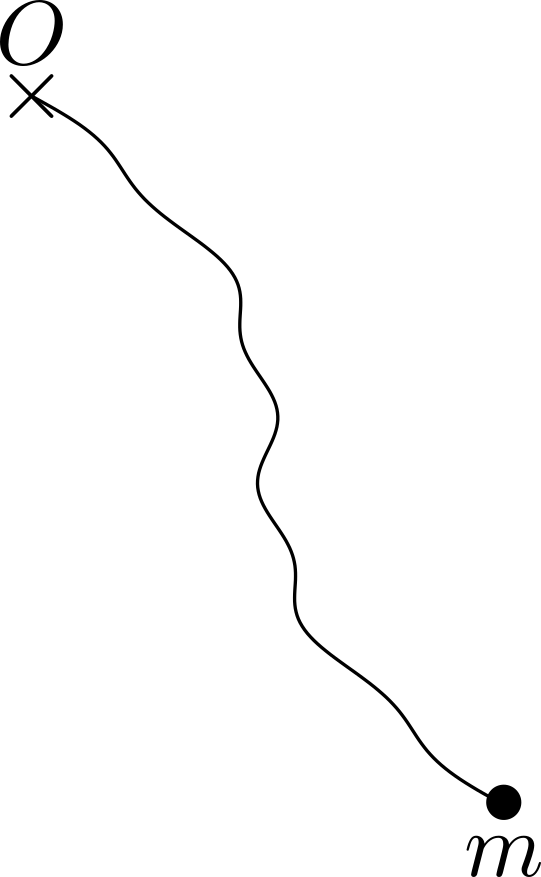
\includegraphics[height=3cm, draft=true]{tension_null}
			}{
				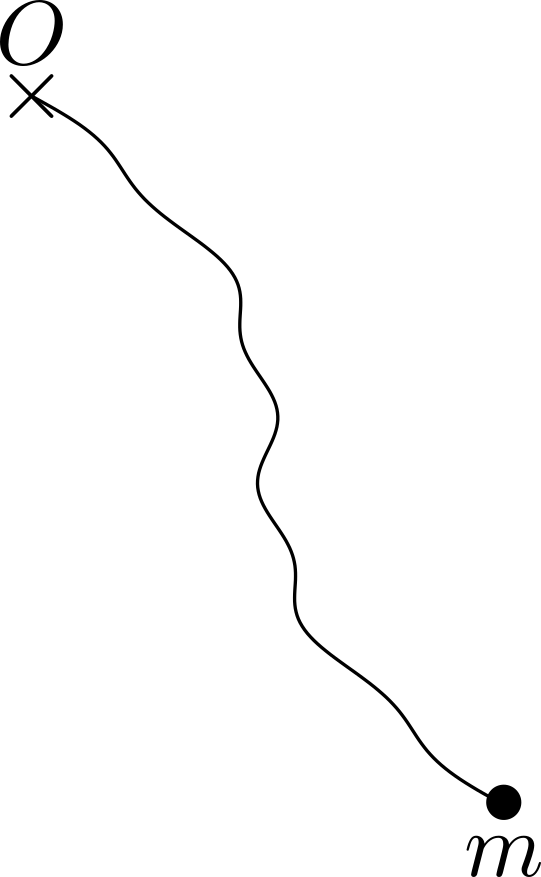
\includegraphics[height=3cm]{tension_null}
			}
			\vspace{-10pt}
			\captionof{figure}{Fil détendu~: pas de force.}
		\end{center}
	\end{minipage}
	\hfill
	\begin{minipage}{0.45\linewidth}
		\begin{center}
			\sswitch{
				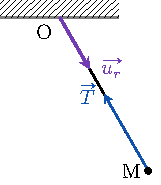
\includegraphics[height=3cm, draft=true]{tension}
			}{
				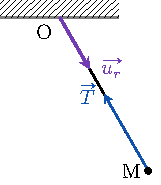
\includegraphics[height=3cm]{tension}
			}
			\vspace{-10pt}
			\captionof{figure}{Fil tendu~: force vers O.}
		\end{center}
	\end{minipage}
\end{tcb*}

\subsection{Pendule simple}
Et si je vous disais qu'on peut mesurer l'attraction de la pesanteur… avec un
bout de ficelle et une masse~?
\bigbreak

\hspace*{-0.75cm}
\begin{minipage}{0.70\linewidth}
	\begin{enumerate}[label=\sqenumi]
		\item[b]{De quoi parle-t-on~?} On étudie le mouvement d'une masse de
		      \SI{20}{g} suspendue à un fil, dans le référentiel du laboratoire
		      supposé galiléen. La masse est écartée de sa position d'équilibre et
		      lâchée sans vitesse initiale.
		\item[b]{Schéma}.
		\item[b]{Modélisation.} On choisit d'utiliser des coordonnées polaires.
		      \begin{itemize}
			      \item La masse est assimilée à un point matériel M.
			      \item Origine~: point d'accroche du fil (centre de rotation
			            pendule).
			      \item Repère~: $(O,\ur,\ut)$ avec base polaire (voir schéma).
			      \item $t$ initial~: moment du lâché, $\th(0) = \th_0$ et
			            $\th(0) = 0$.
		      \end{itemize}
	\end{enumerate}
\end{minipage}
\hfill
\begin{minipage}{0.25\linewidth}
	\begin{center}
		\sswitch{
			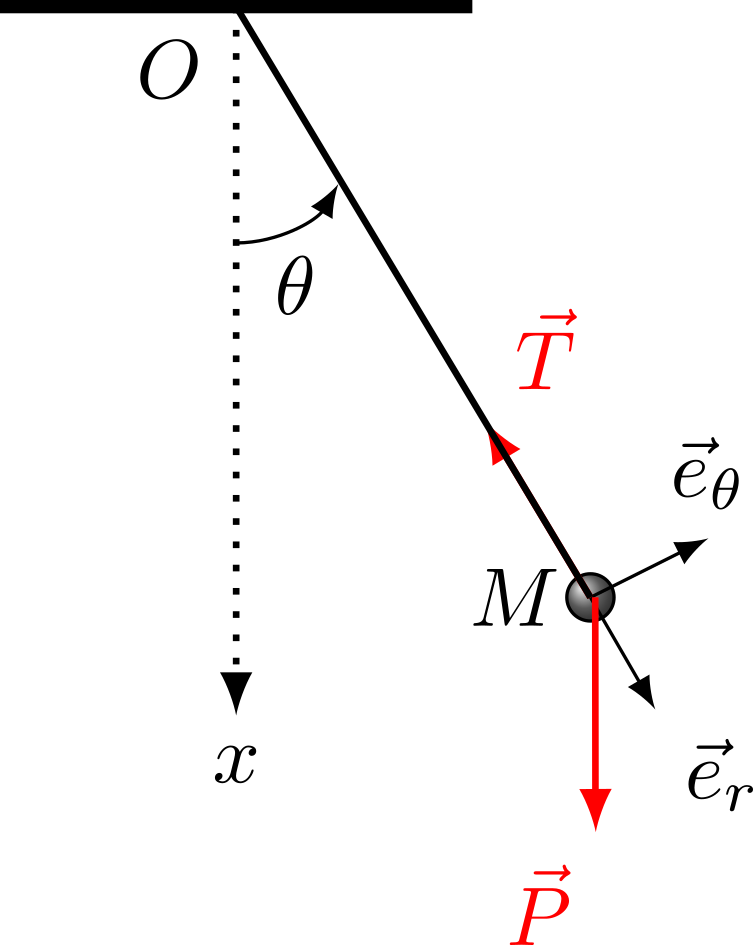
\includegraphics[width=\linewidth, draft=true]{pendule_plain}
		}{
			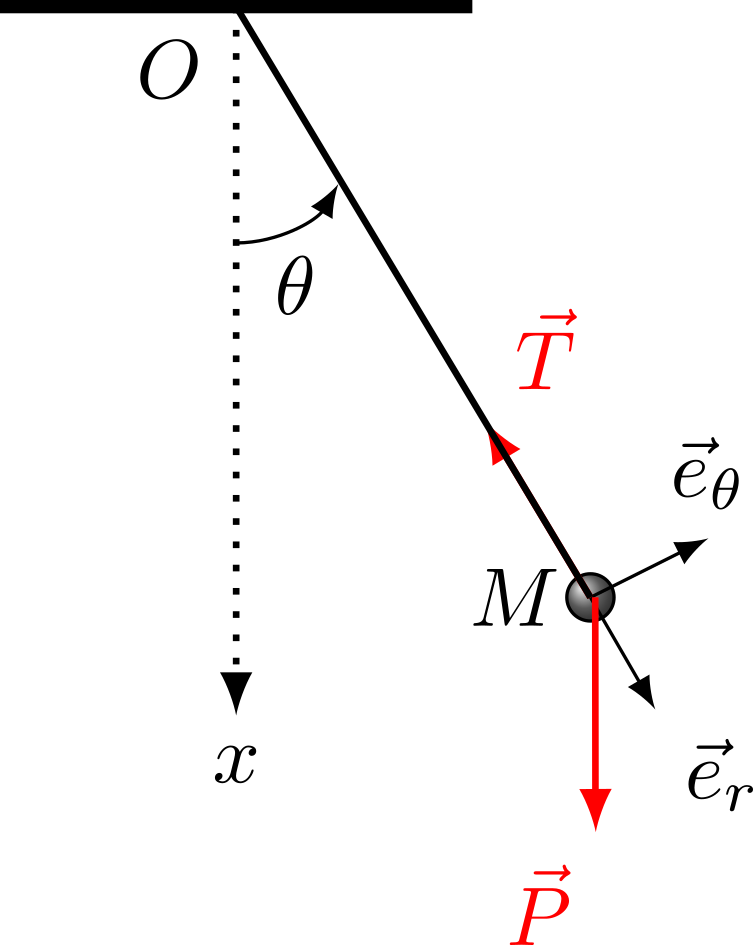
\includegraphics[width=\linewidth]{pendule_plain}
		}
		\vspace{-15pt}
		\captionof{figure}{Schéma}
	\end{center}
\end{minipage}
\begin{enumerate}[label=\sqenumi, start=4]
	\item[b]{Bilan des forces.}
	      \psw{
		      \[
			      \begin{array}{ll}
				      \textbf{Poids}   & \Pf = m\gf = mg(\cos\th \ur - \sin\th \ut)
				      \\
				      \textbf{Tension} & \Tf = -T\ur
			      \end{array}
		      \]
	      }
	\item[b]{PFD.}
	      \psw{
		      \[m\af = \Pf + \Tf\]
	      }
	      Le mouvement étant circulaire (mais pas uniforme), on a
	      \psw{
		      \[\af = -\ell\tp^2 \ur + \ell\tpp \ut\]
	      }
	\item[b]{Équations scalaires.} On projette le PFD sur les axes~:
	      \psw{
		      \[
			      \left\{
			      \begin{array}{rcl}
				      -m\ell\tp^2 & = & mg\cos\th - T \\
				      m\ell\tpp   & = & -mg\sin\th
			      \end{array}
			      \right.
		      \]
	      }
	\item[b]{Résolution.} La première équation n'est pas utilisable telle qu'elle,
	      puisque $T$ n'est pas connue~; cependant la seconde donne une équation
	      différentielle homogène~:
	      \psw{
		      \[\boxed{\tpp + \frac{g}{\ell}\sin\th = 0}\]
	      }
	      qui constitue l'équation du mouvement du pendule. Sous cette forme, elle
	      est \textbf{non-linéaire} donc non résoluble analytiquement~; elle peut
	      l'être numériquement, voir
	      \texttt{Capytale}\footnote{\url{
			      https://capytale2.ac-paris.fr/web/c/a7c5-1241282}}.
\end{enumerate}
En revanche, dans l'approximation des petits angles, on a $\sin\th\approx\th$,
et ainsi on obtient~:
\psw{
	\[\boxed{\tpp + \frac{g}{\ell}\th = 0}\]
}
\textbf{C'est \psw{l'équation différentielle d'un oscillateur harmonique}~!} On
met donc en évidence la pulsation propre
\psw{
	\[\w_0 = \sqrt{\frac{g}{\ell}}\]
}
et on a la solution générale homogène~:
\psw{
	\[\th(t) = A\cos(\w_0t) + B\sin(\w_0t)\]
}
On obtient $A$ et $B$ avec les CI,
\begin{gather*}
	\th(0) = \th_0
	\Lra A\times 1 + B\times 0 = \th_0
	\qdonc
	\boxed{A = \th_0}\\
	\tp(0) = 0
	\Lra -A\w_0\times 0 + B\w_0\times 1 = 0
	\qdonc
	\boxed{B = 0}
\end{gather*}
\leftcenters{et finalement}{\psw{$\boxed{\th(t) = \th_0\cos(\w_0t)}$}}
Le pendule oscille à la pulsation $\w_0$ et à la période $T_0$ telles que
\[
	\w_0 = \sqrt{\frac{g}{\ell}}
	\qet
	T_0 = 2\pi \sqrt{\frac{\ell}{g}}
	\qdonc
	\boxed{g = \psw{\frac{4\pi^2\ell}{T_0{}^2}}}
\]

Dans cette approximation, la période ne dépend \textbf{ni de la masse, ni de
	l'angle initial}. En réalité, si on s'écarte beaucoup de la verticale
($\abs{\theta} > \pi/4$), la période change et n'est plus celle que l'on a aux
petits angles. Voir le changement sur le graphique ci-dessous et en
ligne\footnote{\url{http://www.sciences.univ-nantes.fr/sites/genevieve_tulloue/Meca/Oscillateurs/periode_pendule.php}}.

\begin{minipage}{0.45\linewidth}
	\begin{center}
		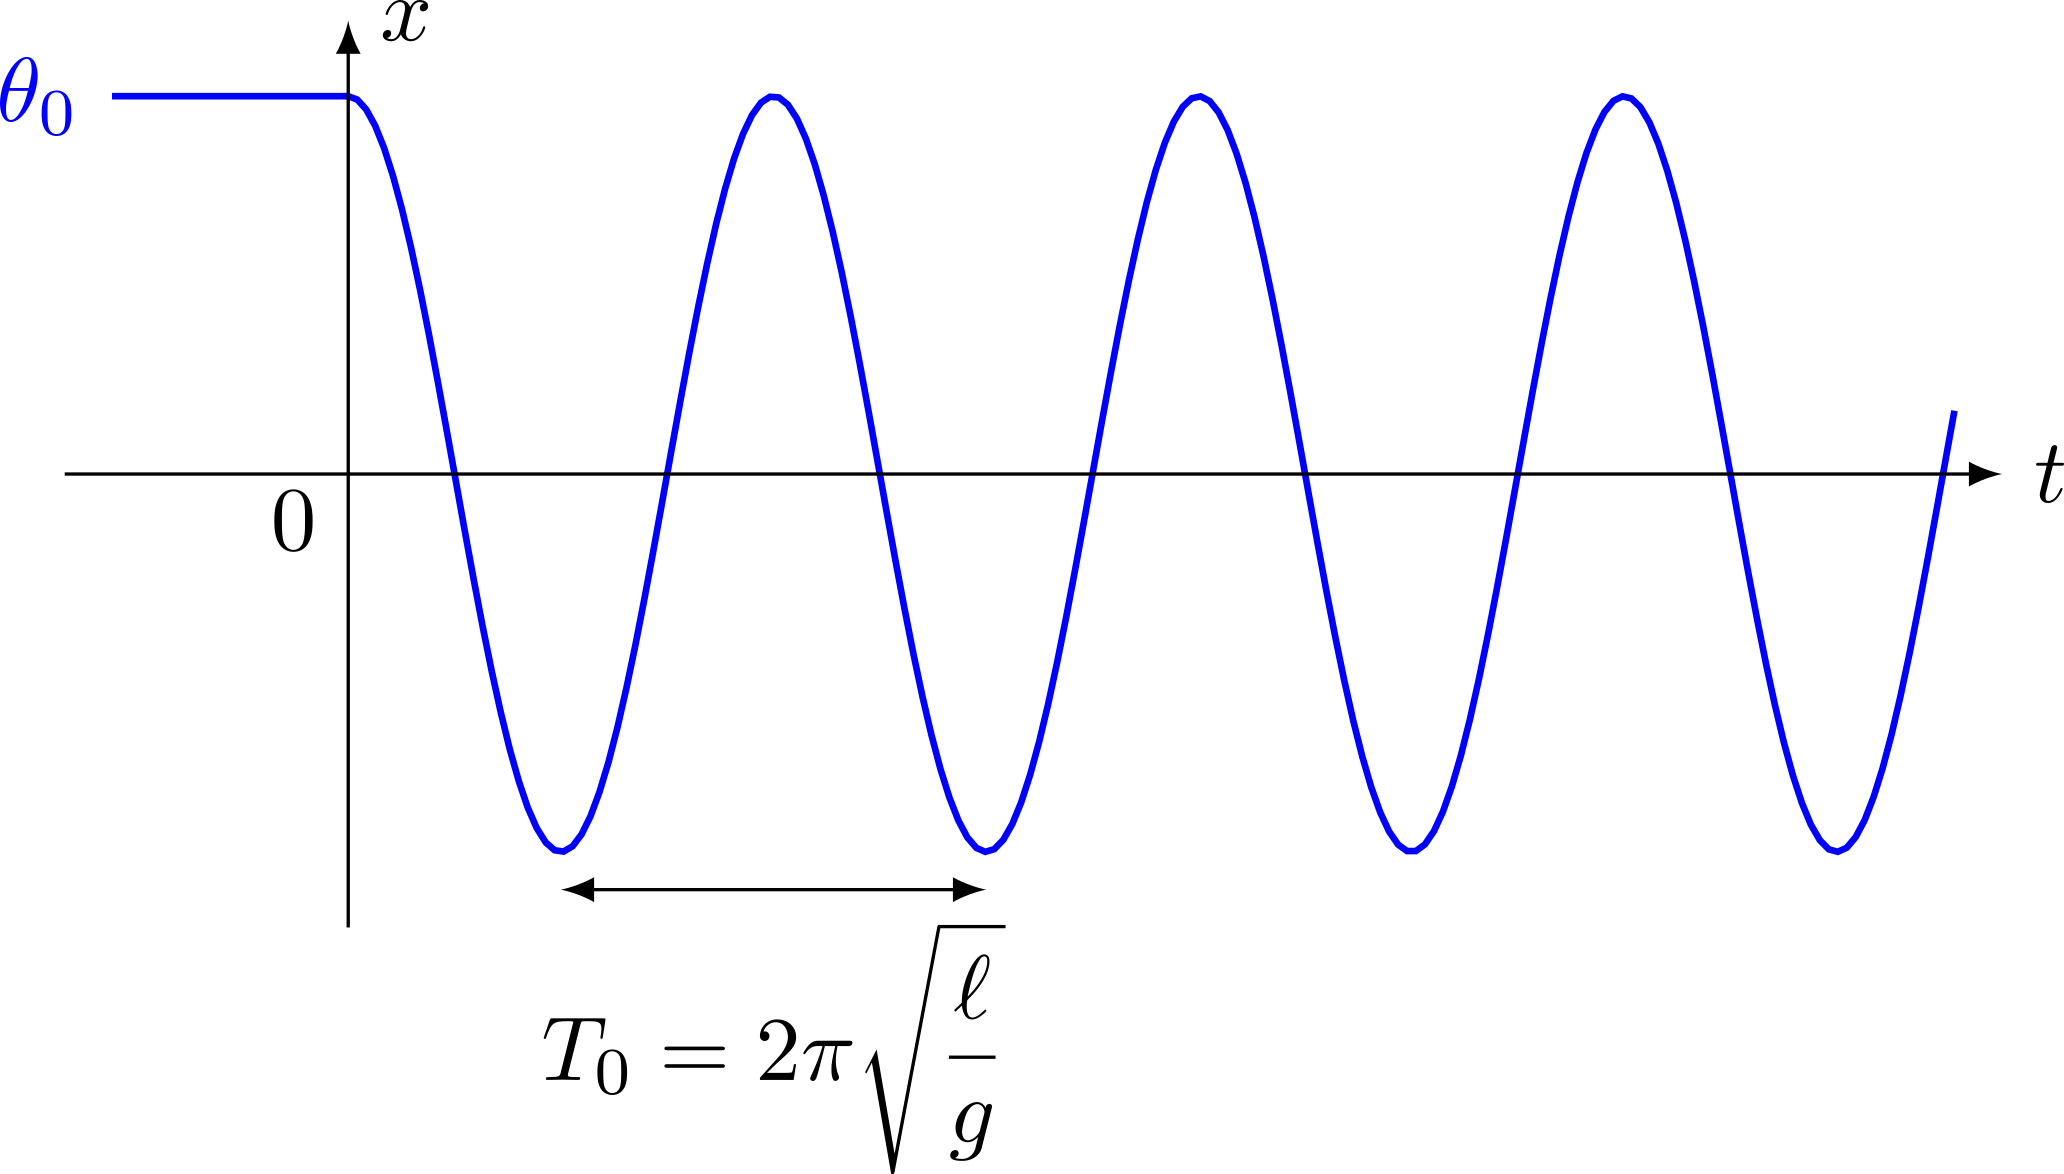
\includegraphics[width=\linewidth]{pendule_sol}
		\captionof{figure}{$\th (t)$ pour petits angles.}
	\end{center}
\end{minipage}
\hfill
\begin{minipage}{0.45\linewidth}
	\begin{center}
		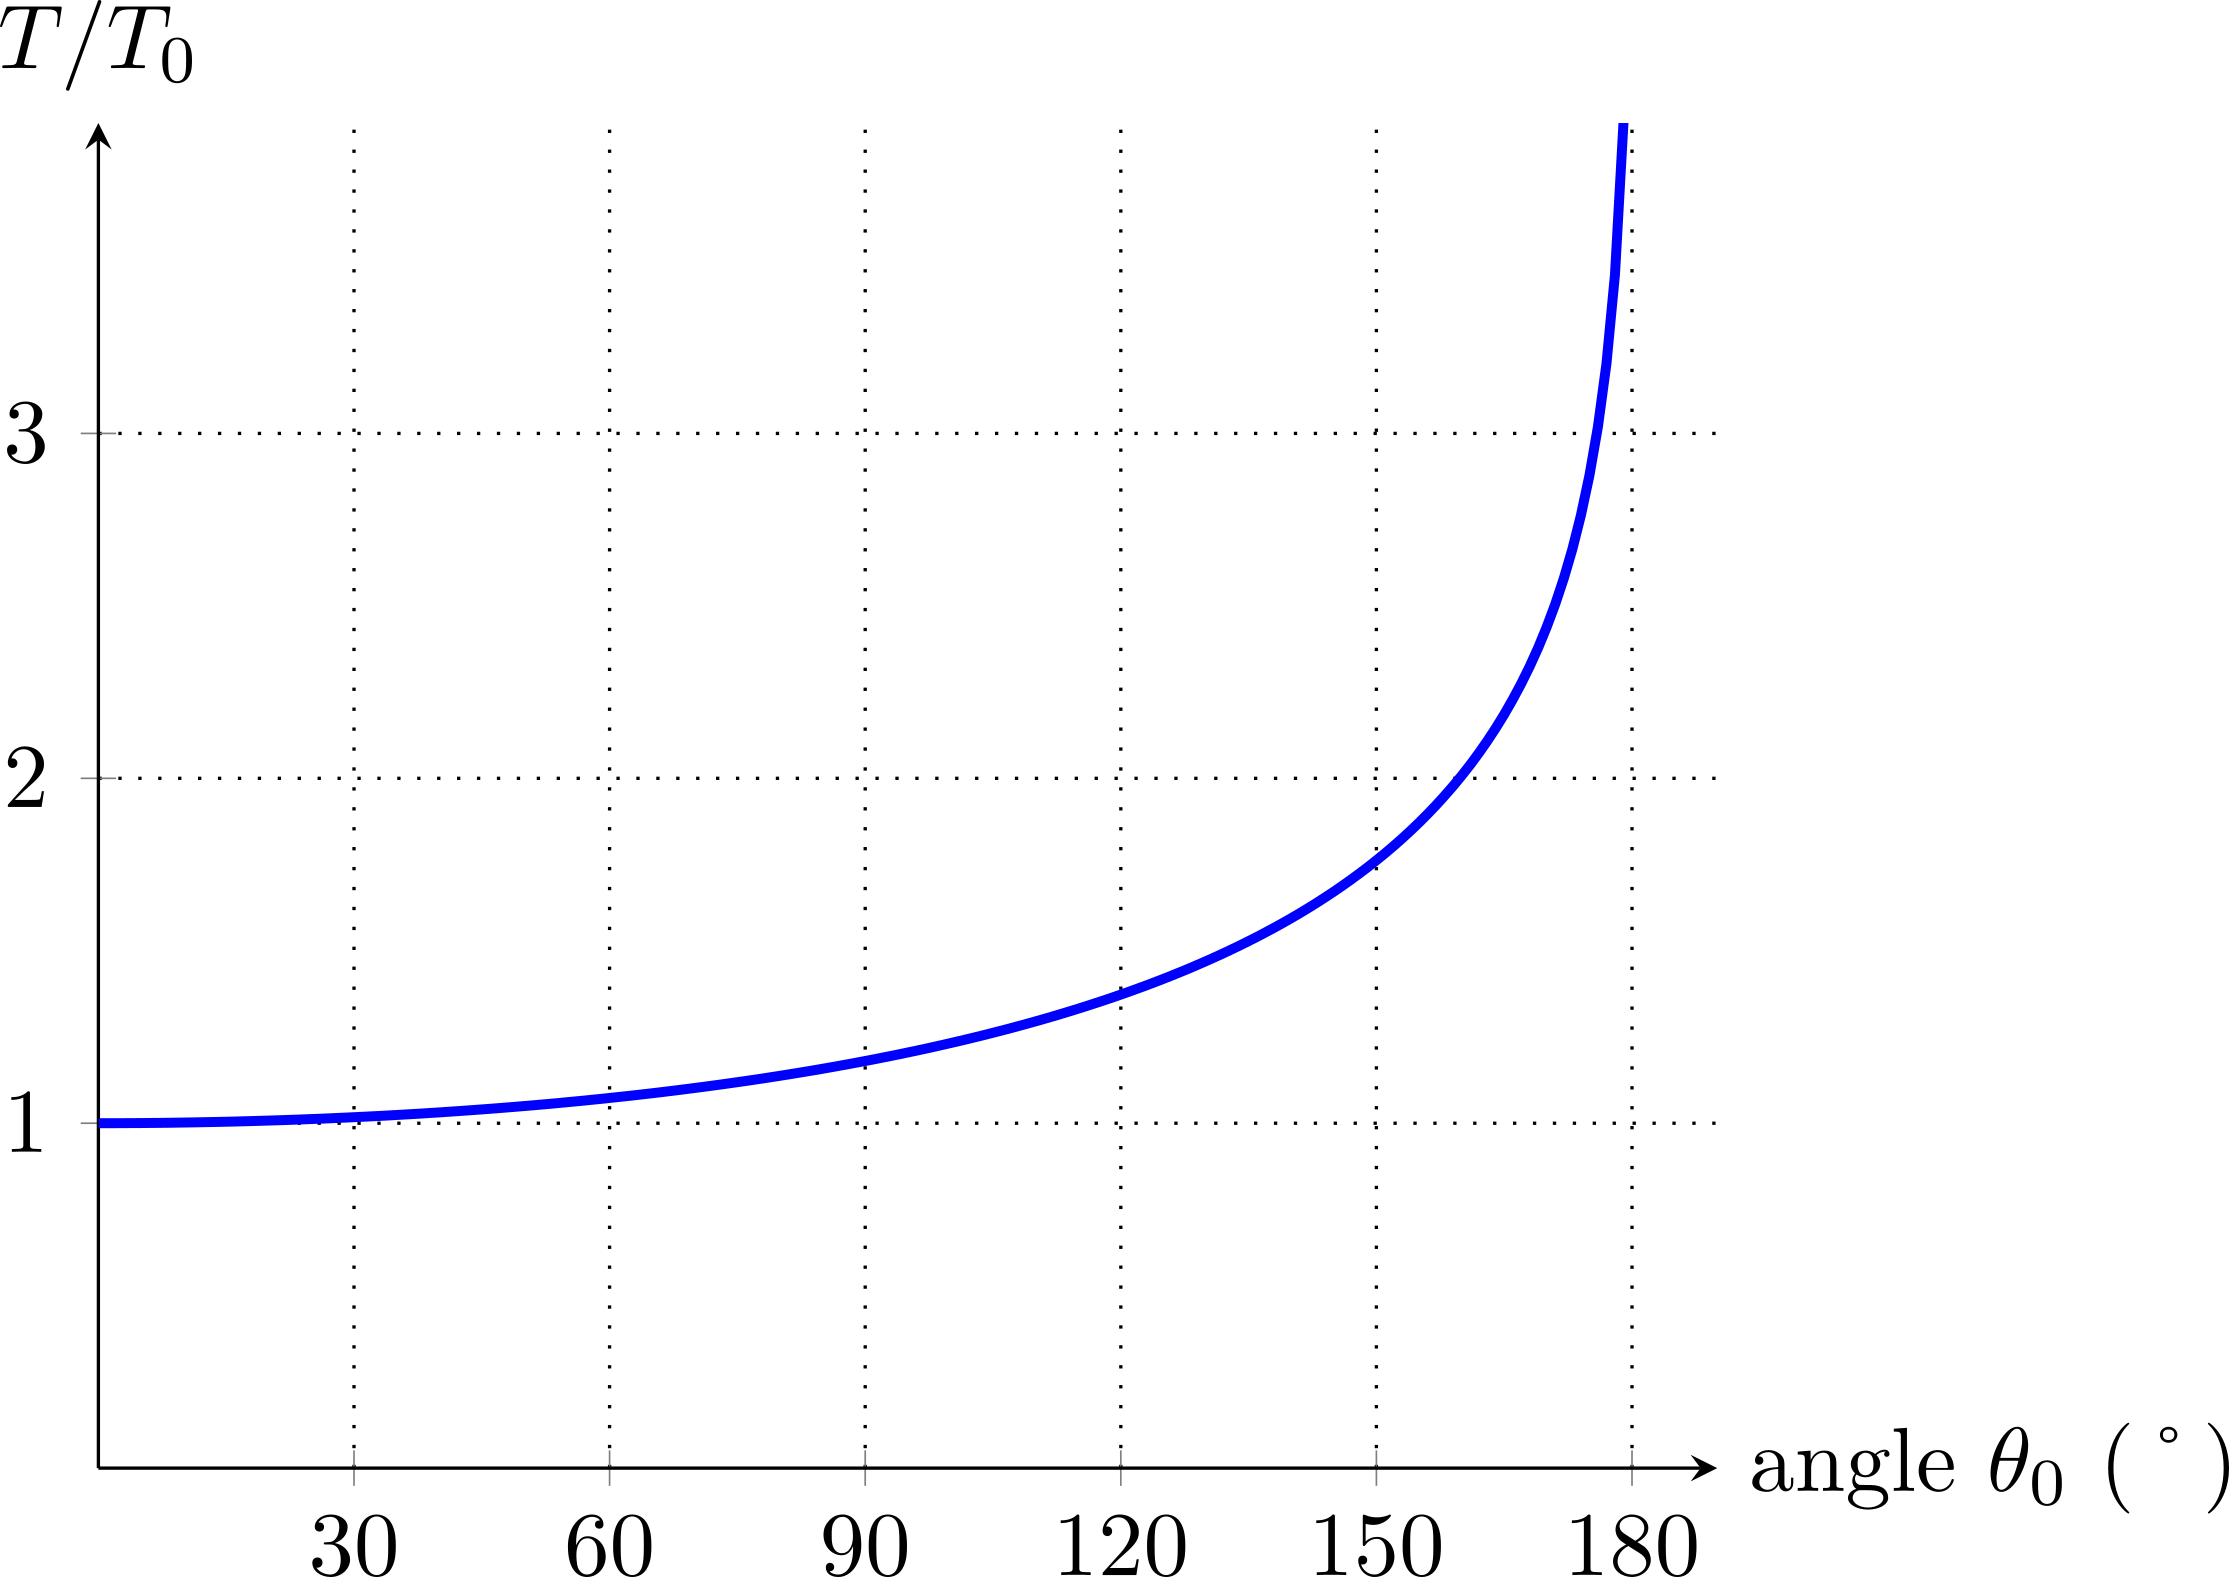
\includegraphics[width=\linewidth]{pendule_gdang}
		\captionof{figure}{Évolution de $T$ selon $\th_0$.}
	\end{center}
\end{minipage}

\begin{tcb*}(appl)<lftt>{Mesure de $g$ par un pendule}
	Ainsi, avec un fil de longueur $\ell = \SI{0.84\pm0.06}{cm}$, on mesure une
	période de $T_0 = \psw{\SI{1.84\pm0.1}{s}}$.
	\smallbreak
	\leftcenters{D'où}{$\boxed{g = \psw{\SI{9.75}{m.s^{-2}}}}$}
\end{tcb*}

\begin{tcb}*(expe)<itc>"trans"{Transition}
	S'il existe de nombreux mouvements plans, il est nécessaire de pouvoir
	décrire des mouvements de rotation qui ne restent pas dans un plan mais
	évoluent dans l'espace 3D.
\end{tcb}

\section{Mouvement courbe dans l'espace}
\subsection{Coordonnées cylindriques}

La manière la plus simple de passer du plan à l'espace est de prendre les
coordonnées polaires et d'y ajouter la coordonnée cartésienne $z$~: on définit
ainsi les coordonnées \textbf{cylindriques}.

\begin{tcb*}[sidebyside, righthand ratio=.25](defi)
	{Repère cylindrique et vecteur position}
	Le repère cylindrique est constitué d'une origine O autour de laquelle sont
	définis trois vecteurs, $(\ur,\ut,\uz)$, avec $(\ur,\ut)$ la base polaire et
	$\uz$ le vecteur de base cartésienne tel que $\ur \wedge \ut = \uz$.
	\bigbreak
	En appelant H le projeté orthogonal de M sur le plan polaire, on a
	\[
		\psw{\boxed{\OM = \vv{\rm OH} + \vv{\rm HM} = r\ur + z\uz}}
		\qet
		\psw{\boxed{\norm{\OM} = \sqrt{r^2 + z^2}}}
	\]
	\tcblower
	\begin{center}
		\sswitch{
			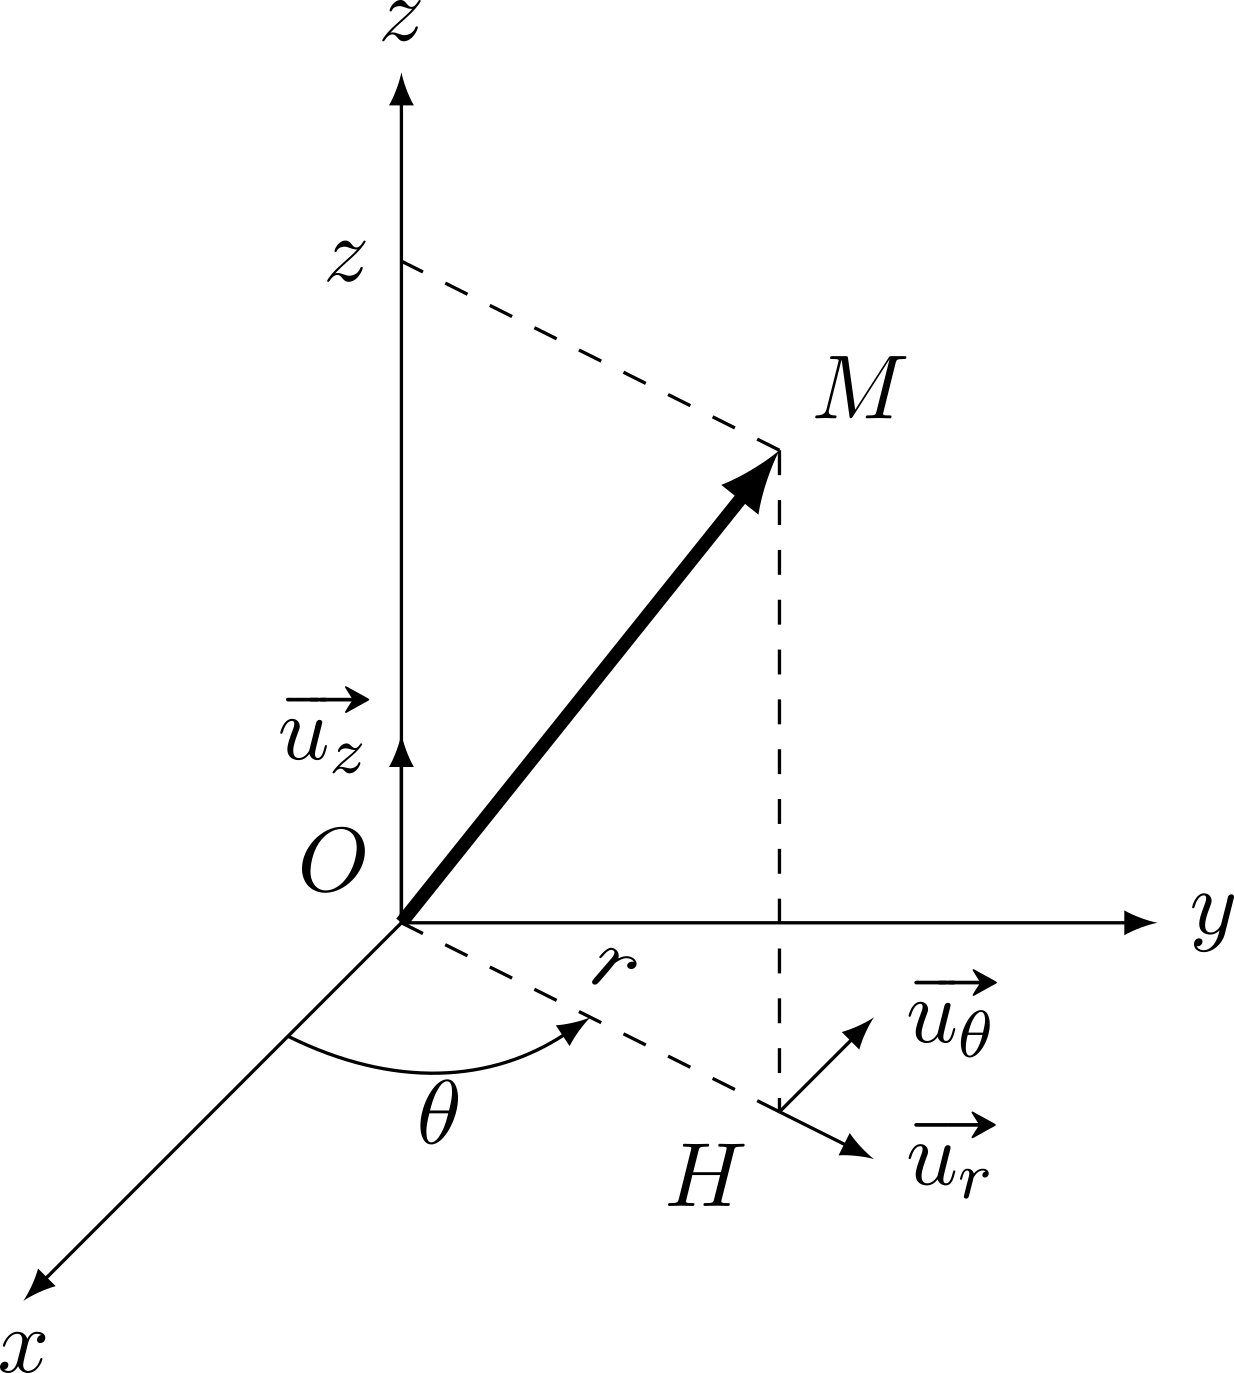
\includegraphics[width=\linewidth, draft=true]{cyl_rep}
		}{
			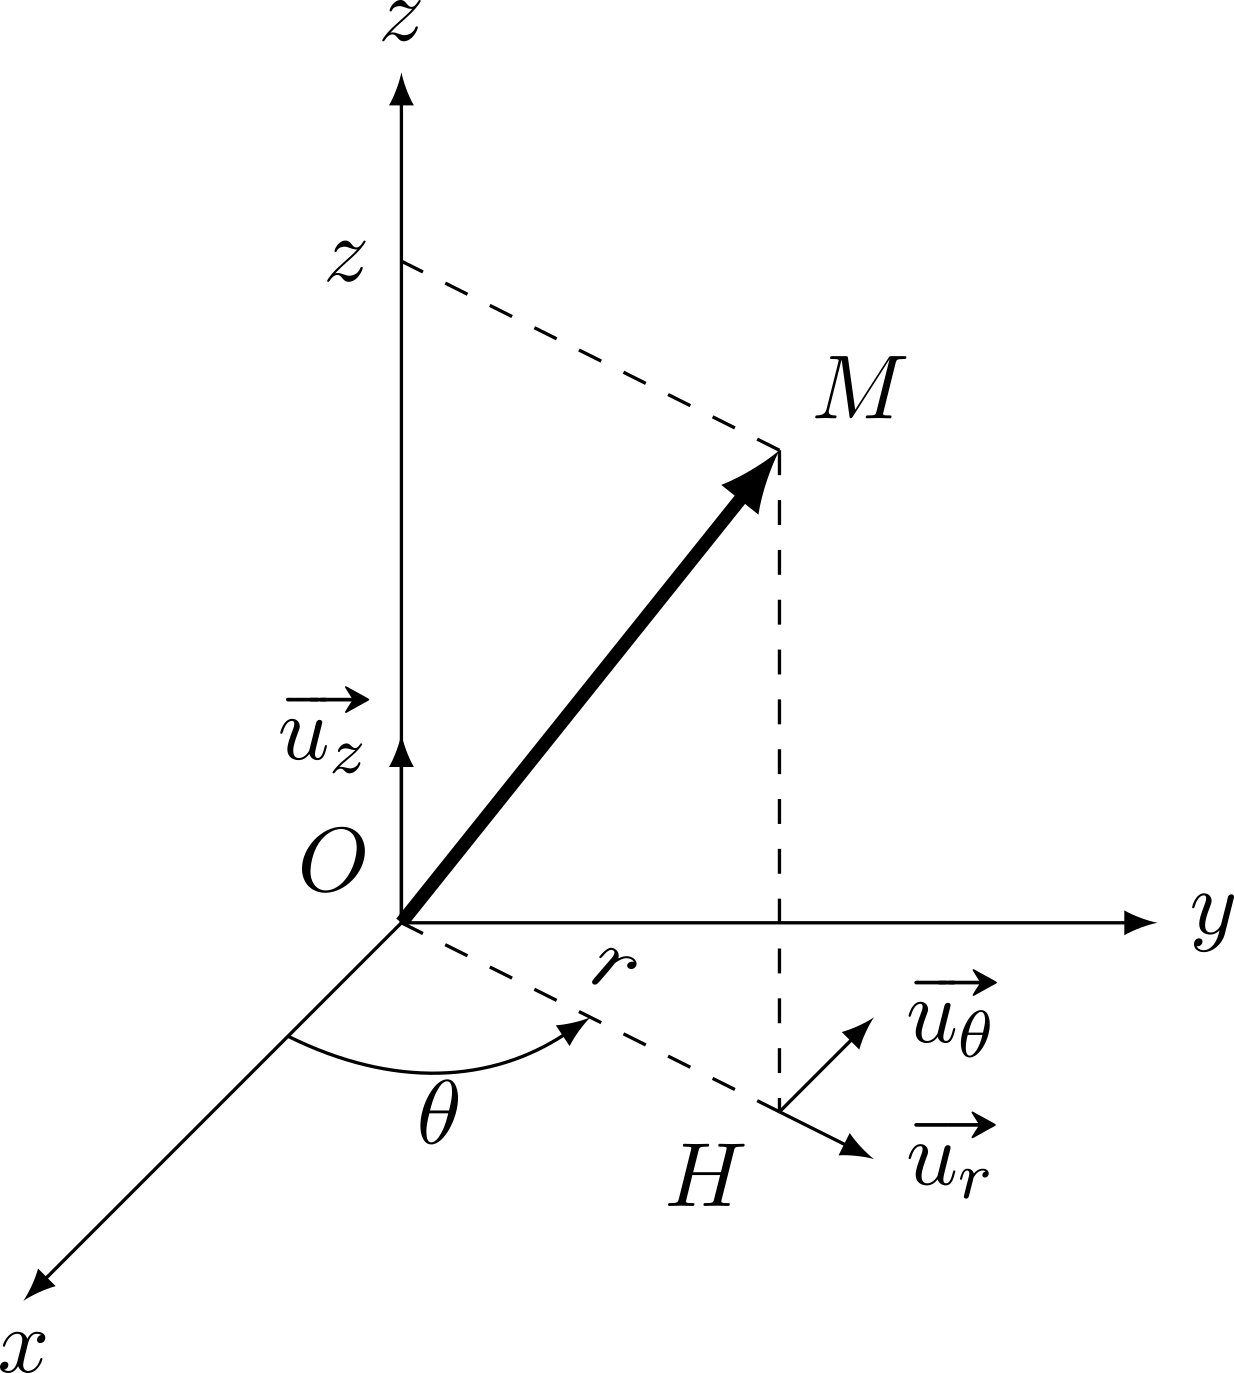
\includegraphics[width=\linewidth]{cyl_rep}
		}
		\vspace{-15pt}
		\captionsetup{justification=centering}
		\captionof{figure}{\smallbreak Cylindriques.}
	\end{center}
\end{tcb*}

La détermination de la vitesse et de l'accélération est la même qu'en polaires,
il suffit d'ajouter les dérivées de $z$ puisque $\uz$ est fixe dans le temps.
Ainsi,

\begin{tcb*}(ror){Bilan~: coordonnées cylindriques}
	\begin{itemize}[itemsep=-10pt]
		\item \leftcenters{\textbf{Coordonnées~:}}
		      {\psw{$(r,\th,z)$}}
		\item \leftcenters{\textbf{Vecteurs de base~:}}
		      {\psw{$(\ur,\ut,\uz)$}}
		\item \leftcenters{\textbf{Position~:}}
		      {\psw{$\OM = r\ur + z\uz$}}
		\item \leftcenters{\textbf{Vitesse~:}}
		      {\psw{$\vf = \rp\ur + r\tp\ut + \zp\uz$}}
		\item \leftcenters{\textbf{Déplacement élém.~:}}
		      {\psw{$\dd\OM = \dd{r}\ur + r\dd{\th}\ut + \dd{z}\uz$}}
		\item \leftcenters{\textbf{Accélération~:}}
		      {\psw{
				      $\DS \af =
					      \left( \rpp -r\tp^2 \right)\ur +
					      \left( 2\rp\tp + r\tpp \right)\ut +
					      \zpp\uz$
			      }}
	\end{itemize}
\end{tcb*}

\noindent
\begin{minipage}{0.48\linewidth}
	Une conséquence fondamentale du déplacement élémentaire est de pouvoir définir
	une surface et un volume infinitésimaux suivant une variation infinitésimale
	des trois coordonnées.
	\smallbreak
	En effet, pour une petite variation $(\dd{r}, \dd{\th}, \dd{z})$,
	on se déplace de $\dd{r}$ dans la direction $\ur$, de $\dd{z}$ dans la
	direction $\uz$ et l'arc de cercle formé par la variation d'angle $\dd{\th}$
	est de longueur $r\dd{\th}$.
\end{minipage}
\hfill
\begin{minipage}{0.25\linewidth}
	\begin{center}
		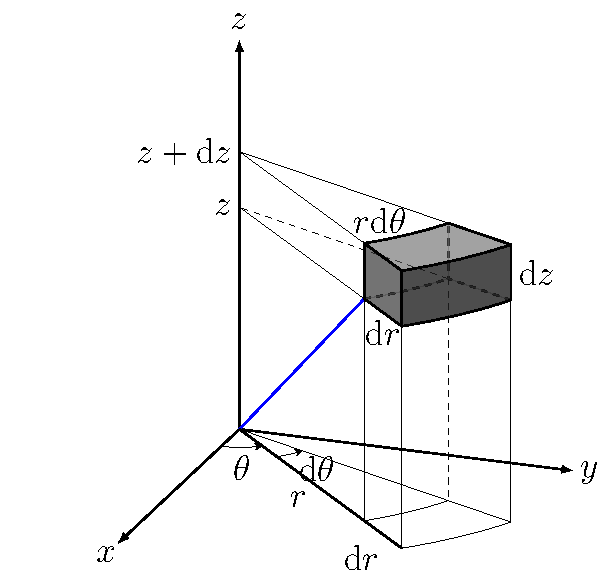
\includegraphics[width=\linewidth]{cyl_vol}
		\captionsetup{justification=centering}
		\captionof{figure}{\\$\dd{V}$ cylindriques.}
	\end{center}
\end{minipage}
\begin{minipage}{0.25\linewidth}
	\begin{center}
		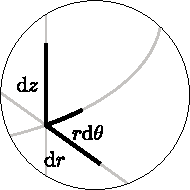
\includegraphics[height=2cm]{zoom_cyl_lgn}
	\end{center}
	\begin{center}
		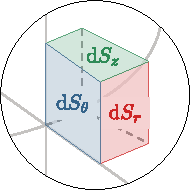
\includegraphics[height=2cm]{zoom_cyl_sfc}
		\captionsetup{justification=centering}
		\captionof{figure}{\\Zoom volume.}
	\end{center}
\end{minipage}

Le volume élémentaire est alors le \textbf{produit de trois composantes de}
$\dd{\OM}$~:
\psw{
	\[
		\boxed{\dd{V} = r \dd{r} \dd{\th} \dd{z}}
	\]
}
On trouve le volume d'un cylindre de rayon $R$ et de hauteur $h$ en
intégrant sur les trois coordonnées~:
\[V\ind{cyl} = \iiint_{r,\th,z} \dd{V} =
	\int_{r'=0}^{R} r'\dd{r'}
	\int_{\th'=0}^{2\pi} \dd{\th'}
	\int_{z'=0}^{h} \dd{z'} =
	\psw{
		\frac{1}{2}R^2\times 2\pi \times h = \boxed{h\pi R^2}
	}
\]
C'est l'aire d'un disque multiplié par la hauteur~!

\begin{tcb*}(impo){Choix des coordonnées}
	Dans un problème de mécanique, on choisit les coordonnées judicieusement en
	fonction des symétries du système. \textbf{Sauf proposition de l'énoncé}, on
	utilisera les coordonnées \textbf{cylindriques} pour les mouvements de
	\textbf{rotation}. On utilisera les coordonnées cartésiennes sinon.
\end{tcb*}

\subsection{Coordonnées sphériques}
La manière la plus complète de décrire un mouvement général dans l'espace repose
sur un dernier système de coordonnées, les coordonnées \textbf{sphériques}.

\begin{tcb*}(defi){Repère sphérique}
	\begin{isd}[righthand ratio=.28]
		Le repère sphérique est constitué d'une origine O autour de laquelle sont
		définis trois vecteurs, $(\ur, \ut, \uf)$, tels que
		\[\boxed{\OM = r\ur}
			\qavec
			\boxed{\th = \widehat{(\uz,\OM)}}
			\qet
			\boxed{\f = \widehat{(\ux,\vv{\rm OP})}}
		\]
		où $\widehat{(\cdot, \cdot)}$ est l'\textbf{angle orienté}, et P le
		projeté orthogonal de M sur le plan polaire. \textbf{$\mathbf{\f}$
			correspond à $\th$ des coordonnées polaires.}
		\tcblower
		\begin{center}
			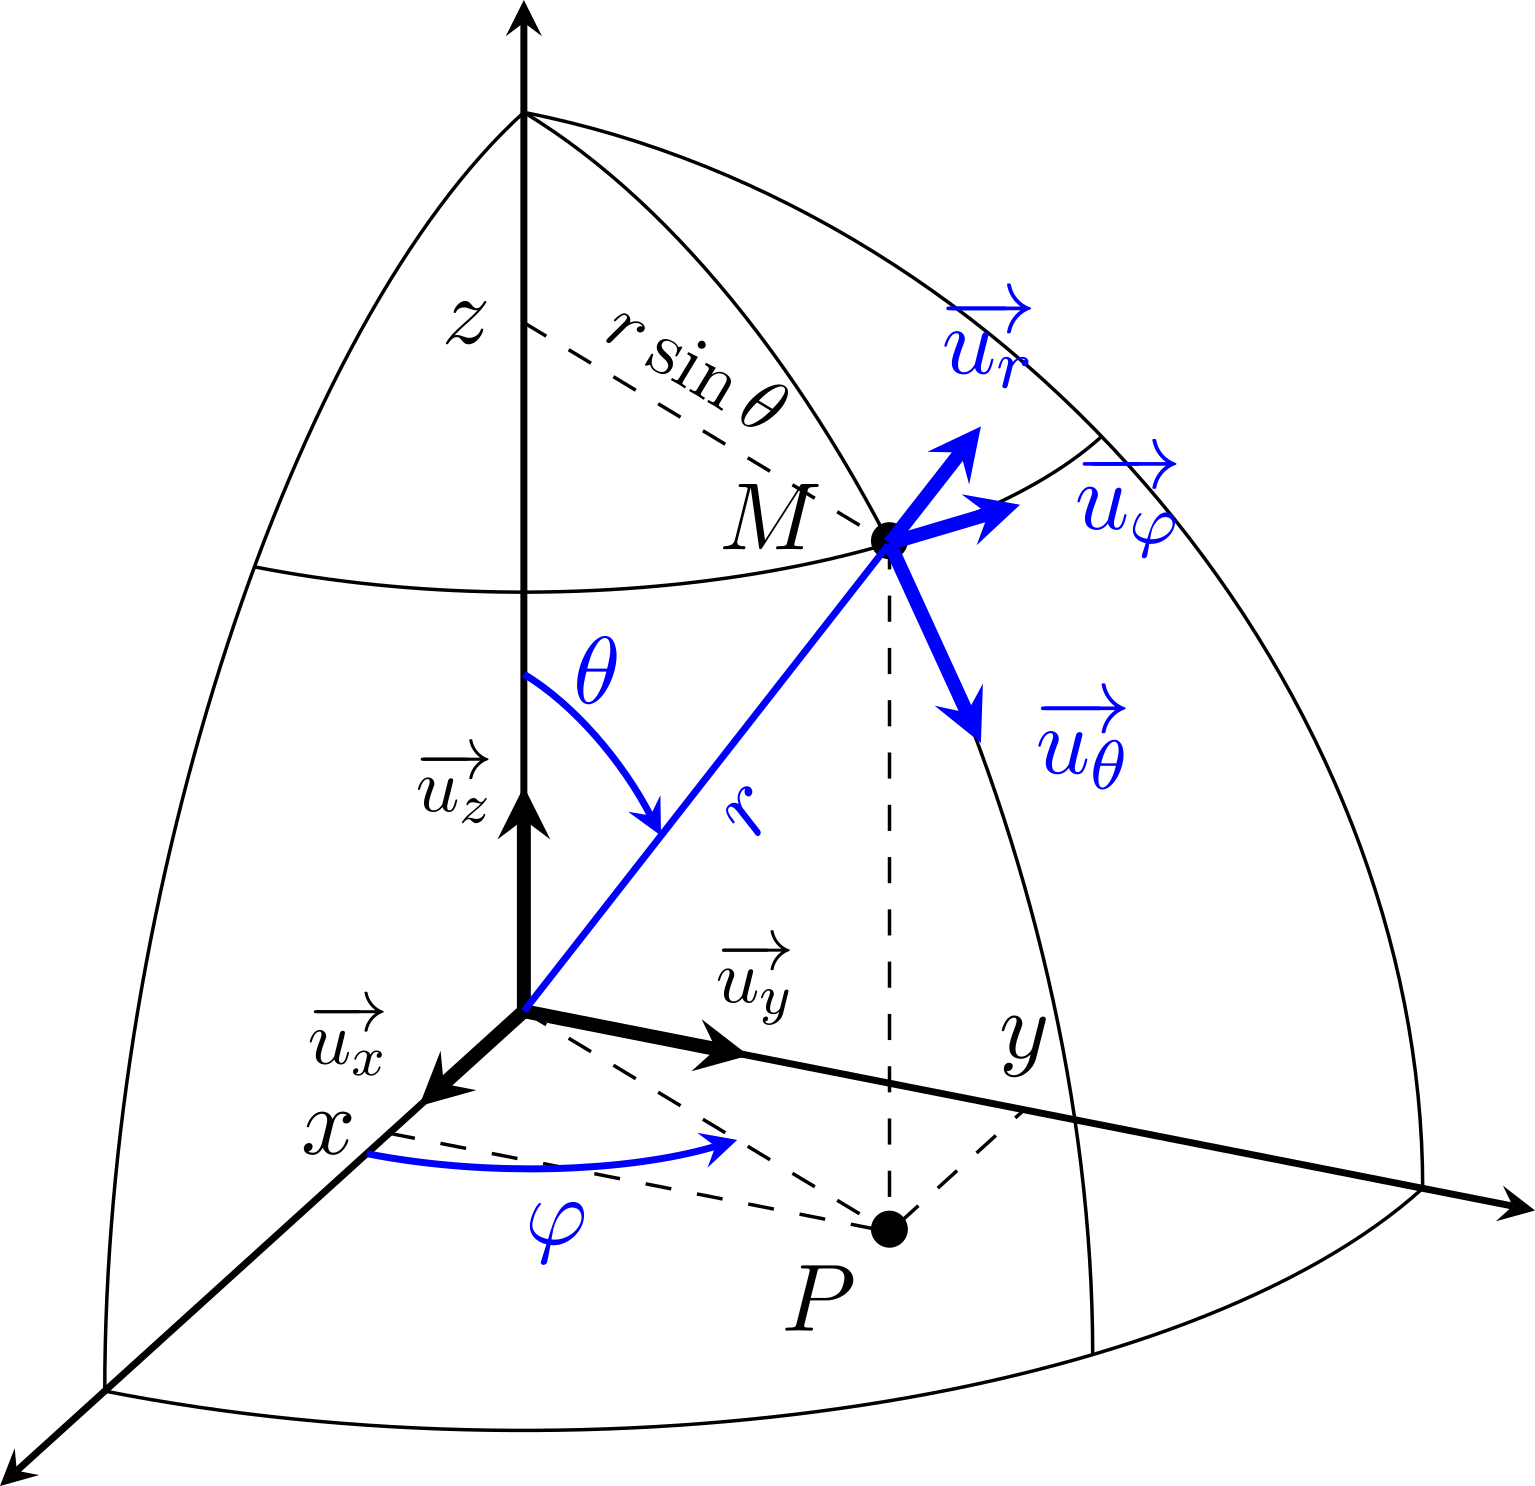
\includegraphics[width=\linewidth]{sph_rep}
			\captionsetup{justification=centering}
			\captionof{figure}{\\Sphériques.}
		\end{center}
	\end{isd}
	\begin{itemize}[itemsep=-5pt]
		\item $\th \in [0~;~\pi]$ est nommé \textbf{colatitude} ($\lb =
		      \abs{\pi/2 - \th}$ la latitude)~, et respecte
		      \[  \tan\th
			      = \frac{\rm OP}{z}
			      \Lra \th
			      = \arctan(\frac{\sqrt{x^2 + y^2}}{z})
		      \]
		\item $\f \in [0~;~2\pi]$ est nommé \textbf{longitude}, et respecte $\DS
			      \f = \arctan(\frac{y}{x})$.
	\end{itemize}
\end{tcb*}

\begin{itemize}
	\item Une courbe $\th = \cte$ est appelée \textbf{parallèle}~; le
	      \textbf{rayon} d'un parallèle est \fbox{$r\sin\th$}.
	\item Une courbe $\f = \cte$ est appelée \textbf{méridien}~; le
	      \textbf{rayon} d'un méridien est \fbox{$r$}.
\end{itemize}

On peut inverser les définitions en prenant $x = {\rm OP}\cos\f$ et $y = {\rm
	OP}\sin\f$, pour avoir
\[
	\boxed{x = r\sin\th\cos\f}
	\quad,\quad
	\boxed{y = r\sin\th\sin\f}
	\qet
	\boxed{z = r\cos\th}
\]

\begin{tcb*}(exem)<lftt>{Repérage sphérique sur Terre}
	\begin{minipage}{0.70\linewidth}
		Le repérage sur la Terre utilise la latitude et la longitude. Par
		exemple, le lycée \textsc{Pothier} se situe à \ang{47.90}N,
		\ang{1.90;;}E~; on a donc
		\[
			\th\ind{\textsc{Pothier}} = \ang{42.1}
			\qet
			\f\ind{\textsc{Pothier}} = \ang{1.90}
		\]
	\end{minipage}
	\hfill
	\begin{minipage}{0.25\linewidth}
		\begin{center}
			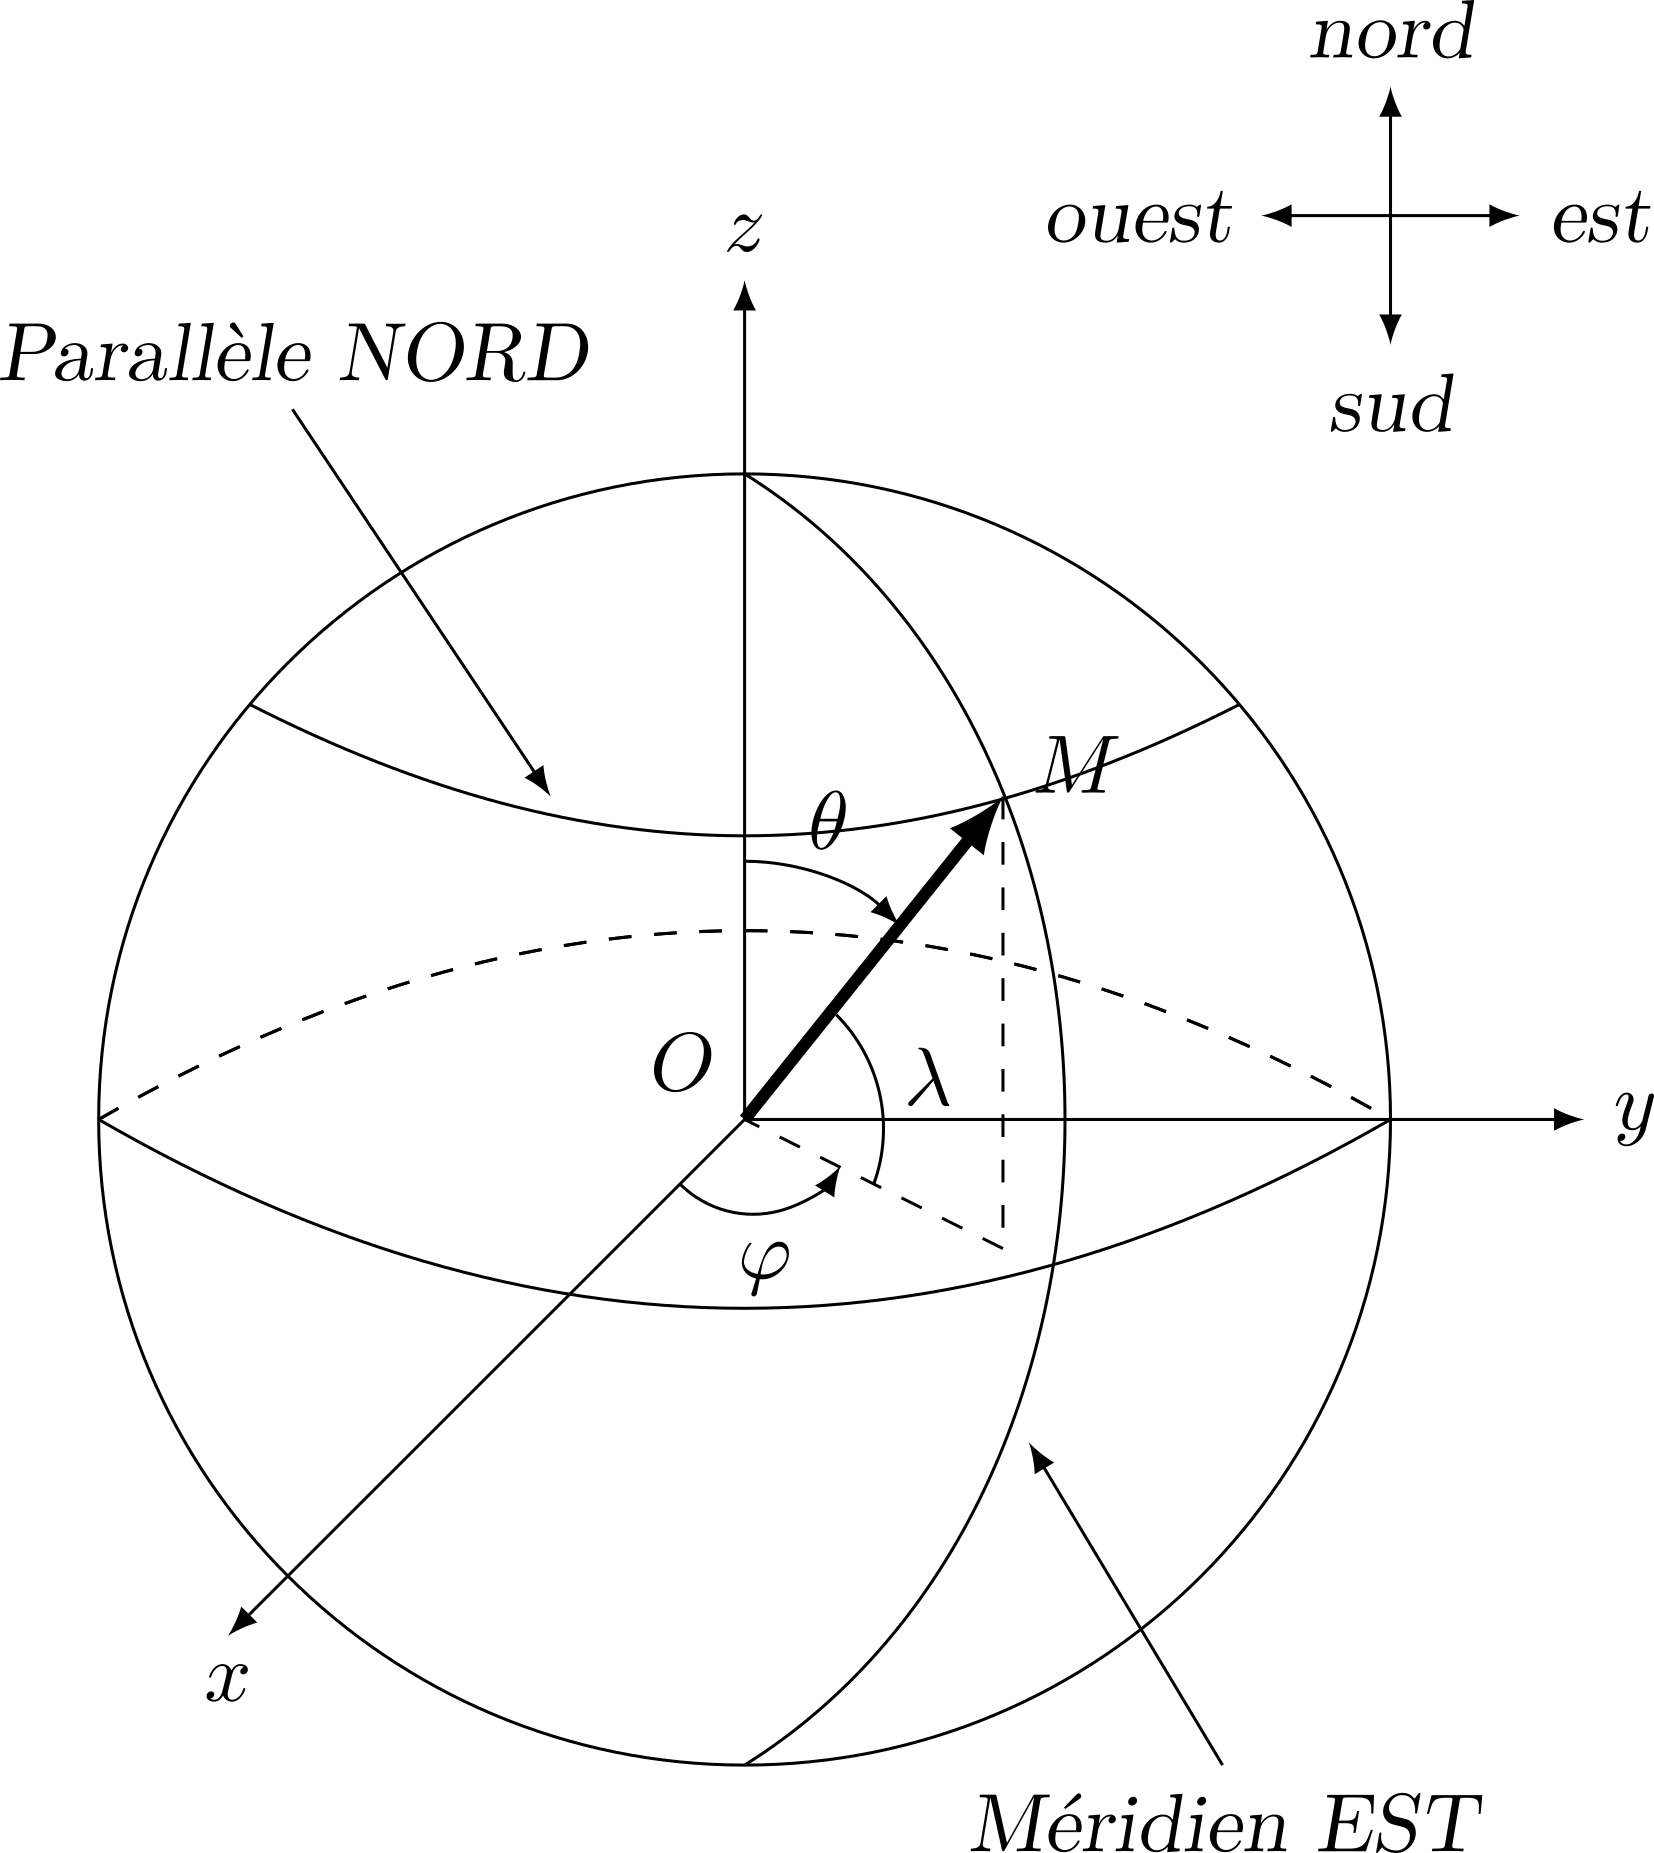
\includegraphics[width=\linewidth]{sph_terre}
		\end{center}
	\end{minipage}
\end{tcb*}


\begin{tcb*}[sidebyside, righthand ratio=.5](prop)
	{Déplacement élémentaire sphérique}
	\begin{itemize}
		\item Variation $\dd{r}$ $\Ra$ déplace\mnt\ $\dd{r}\ur$~;
		\item Variation $\dd{\th}$ $\Ra$ déplace\mnt\ $r\dd{\th}\ut$~;
		\item Variation $\dd{\f}$ $\Ra$ déplace\mnt\ $r\sin\th\dd{\f}\uf$.
	\end{itemize}
	\[\boxed{\dd\OM = \dd{r}\ur + r\dd{\th}\ut + r\sin\th\dd{\f}\uf}\]
	\tcblower
	\noindent
	\begin{minipage}{.59\linewidth}
		\begin{center}
			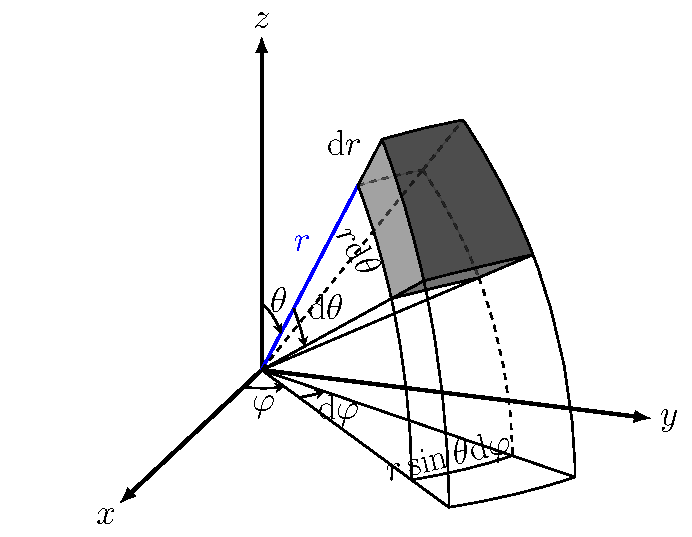
\includegraphics[width=\linewidth]{sphe_vol}
			\captionsetup{justification=centering}
			\captionof{figure}{\\$\dd{\protect\OM}$ sphériques}
		\end{center}
	\end{minipage}
	\begin{minipage}{.39\linewidth}
		\begin{center}
			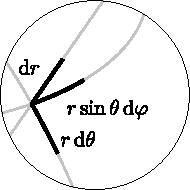
\includegraphics[height=2cm]{zoom_sph_lgn}
		\end{center}
		\begin{center}
			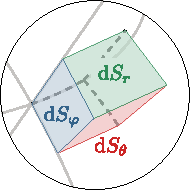
\includegraphics[height=2cm]{zoom_sph_sfc}
			\captionsetup{justification=centering}
			\captionof{figure}{Zoom volume.}
		\end{center}
	\end{minipage}
\end{tcb*}

On trouve de la même manière le volume élémentaire~:
\psw{
	\[
		\boxed{\dd{V} = r^{2}\sin(\theta)\dd{r}\dd{\th}\dd{\f}}
	\]
}
Il permet de déterminer le volume d'une boule~:
\[
	V\ind{boule}
	= \iiint_{r,\th,\f}
	= \int_{r'=0}^{R} r'^2\dd{r'}
	\int_{\th' = 0}^{\pi} \sin\th'\dd{\th'}
	\int_{\f'=0}^{2\pi} \dd{\f}
	= \int_{r'=0}^{R} 4\pi r'^2 \dd{r}
	\psw{
		= \boxed{\frac{4}{3}\pi R^3}
	}
\]

\end{document}
